\documentclass[runningheads]{llncs}

\usepackage{graphicx}
% Used for displaying a sample figure. If possible, figure files should
% be included in EPS format.
\usepackage{float}

\begin{document}
%
\title{Simulation Paper}

\author{Benjamin Vandersmissen\inst{1} \and
Lars Van Roy\inst{2} \and \\
Evelien Daems\inst{3} \and
Frank Jan Fekkes\inst{4}}
%
\authorrunning{B. Vandersmissen, L. Van Roy, E. Daems, F.J. Fekkes}
% First names are abbreviated in the running head.
% If there are more than two authors, 'et al.' is used.
%
\institute{
\email{benjamin.vandersmissen@student.uantwerpen.be} \and
\email{lars.vanroy@student.uantwerpen.be} \and
\email{evelien.daems@student.uantwerpen.be} \and
\email{franciscus.fekkes@student.uantwerpen.be}}
%
\maketitle              % typeset the header of the contribution
%
\begin{abstract}
In this paper we will examine the Stride tool and discover its functionalities.
We will discuss some findings about the use of different parameters, populations and more.
In the end there is a brief discussion of the performance of the program, a very important topic within computer related problems.

%\keywords{First keyword  \and Second keyword \and Another keyword.}
\end{abstract}

\section{Simulation}

\subsection{Stochastic variation}
We use the Stan (STochatsic ANalysis) controller to examine the influence of stochasticity on the results obtained from the simulation. \\ \\
In Figure \ref{fig1} the number of cummulative cases per time-step is plotted. Here we can observe an exponential grow of the number of cases througout time. This is not surprisingly because it can be deducted from common reasoning. If per time more people are affected, a larger contactpool is possibly infected. These people who are now new carriers of the disease will enter their personal contactpool and again more people will be reached.\\ \\
Towards the end a flattening of the curve occurs. This is not something totally unexpected because the population is obviously not infinite. At one point anyone who can be infected will effectively become a carrier of the disease.\\ \\
The same reasoning can explain the curve in Figure \ref{fig2}. Now the cases are not the cummulative ones but the number of new cases in each time-step. A similar course of the curve can be observed.

\begin{figure}
	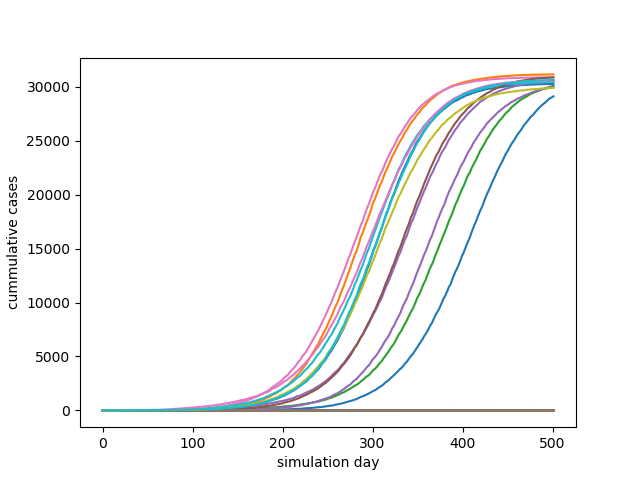
\includegraphics[width=\textwidth]{fig1.png}
	\caption{Result of a number of stochastic runs. The figure displays the distribution of the number of cummulative cases per time-step.} 	
	\label{fig1}

	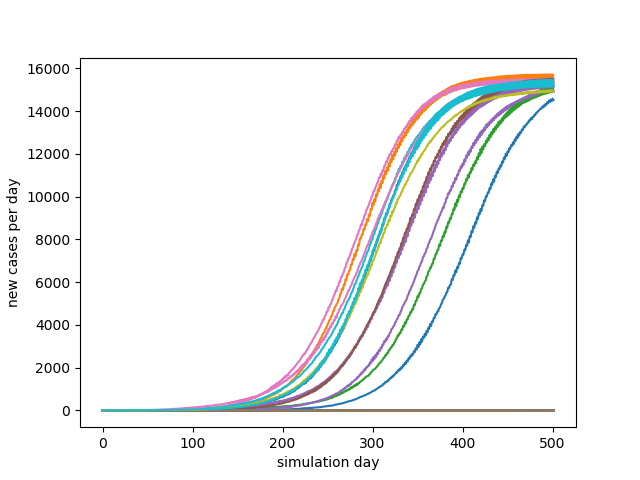
\includegraphics[width=\textwidth]{fig2.png}
	\caption{Result of a number of stochastic runs. The figure displays the distribution of the number of new cases per time-step.} 
	\label{fig2}
\end{figure} 
\newpage


\subsection{Determining an extinction threshold}
In the previous section 1.1 (Stochastic variation) we found that extinction will influence the outcome. It is neccessary to be able to exclusively look at outbreaks. If we can find some threshold where there is a clear difference between large outbreaks and extinctions we can seperate the two scenarios.\\ \\
After running fifty simulations we can plot the total number of infected cases and their frequency.  We used the file "stochastic\_analysis.xml" for the simulations. After running the simulator the outcome is plotted in the histogram in Figure \ref{fig3} where the frequency of the amount of infected cases is plotted.\\ \\
There is a clear distinction between large outbreaks and smaller ones. Be The smaller ones are again plotted in the second histogram "extinction\_small.jpg". There it can be noticed that small outbreaks are really small (20 maximum). Which can be called an extinction after 500 days. The threshold for this example can be set between than 50 and 25 000. Either of those thresholds should eliminate all extinctions in this case.\\ \\
A very low threshold might allow some extinctions to be passed while a high threshold might eliminate an outbreak. What can be noticed is the total lack of simulations between 100 and 25000 infected cases. But there can still be exceptions in the infected cases. A threshold of 1000 would be more than adequate. It will eliminate all extinctions while keeping the outbreaks.\\ \\
It should be noted that this threshold will change for a lot of variables. For example: time and population will affect the threshold. A new threshold should be determined for each set of simulations.

\begin{figure}
	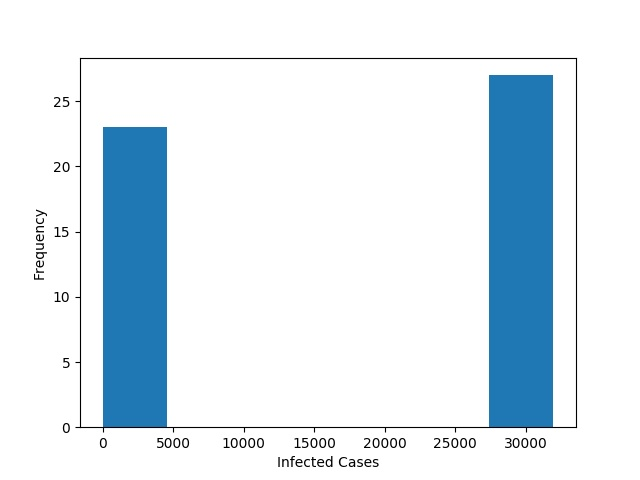
\includegraphics[width=\textwidth]{extinction_all.jpg}	
	\caption{Above is an histogram with the frequency of total infected cases for 50 simulations. 5000 cases can be seen as a small outbreak see fig \ref{fig4} for an enlargement of the left spike.}
	\label{fig3}
	
	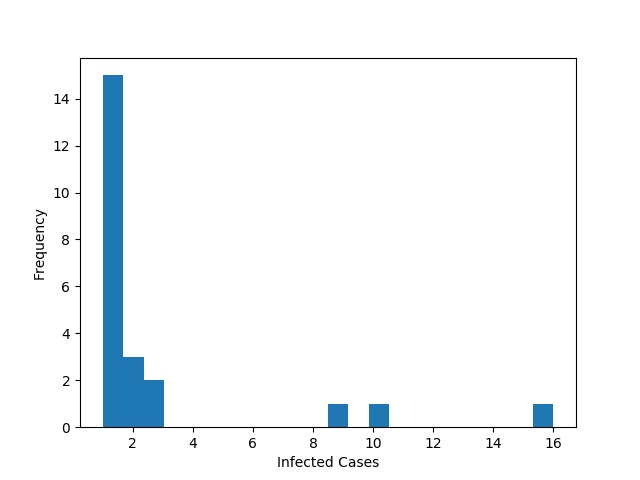
\includegraphics[width=\textwidth]{extinction_small.jpg}
	\caption{A zoom on the left spike of figure \ref{fig3}. Instead of 0 to 5000 it is actually 0 to 16.}	
	\label{fig4}
\end{figure}
\newpage

\subsection{Estimating the immunity level}
For this assignment we had to estimate the percentage of people who were immune to the disease given the following graph.
\\ 
\begin{figure}[h!]
	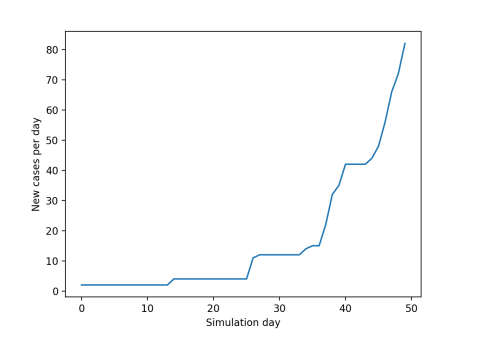
\includegraphics[width=\textwidth]{original.png}
	\caption{New cases observed per day during the outbreak}
\end{figure}
\newpage
As a first approximation we performed 10 simulations with immunity levels ranging from 0 to 90\% as seen in the next graph. As we can clearly see, all immunity levels lower then 50\% are unrealistic, compared to the desired graph. As a next step we decided to drop off the unrealistic immunity levels and generated a zoom of the realistic immunity levels with the same offset.
\begin{figure}
	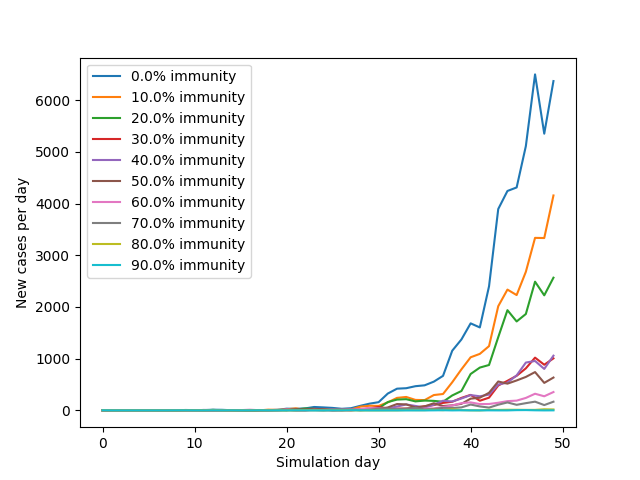
\includegraphics[width=\textwidth]{test_immunity_0-100.png}
	\caption{first estimate of outbreaks}
\end{figure}
\newpage

\newpage
\noindent
By dropping all percentages lower than 60 and higher than 90\% we get the following graph, this graph is a lot closer to the desired graph (since the highest number of new cases is now only 110 compared to over 6000), but is still far from accurate. We can now see that the desired immunity rate should lie somewhere between 70 and 80\% as 70 is too high and 80 is too low.
\begin{figure}
	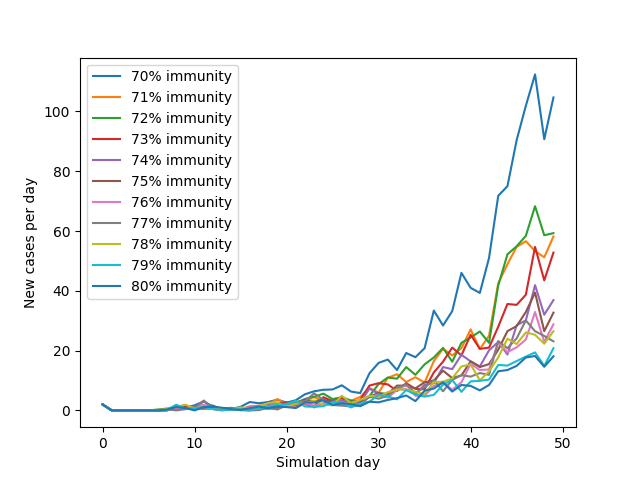
\includegraphics[width=\textwidth]{test_immunity_70-80.png}
	\caption{narrowed down estimate of outbreaks based on 10 simulations}
\end{figure}

\newpage
\noindent
Finally, we zoom in between 70 and 75\% and we can see that the immunity percentage is somewhere around the 70\% mark. Curiously enough, with an immunity rate of 71\% and an average of 25 simulations, there are more infected than with an immunity rate of 70\%. The only problem with this 70 \% graph is that there is a sudden drop in infections around day 45 while the original graph doesn't feature that drop.
\begin{figure}
	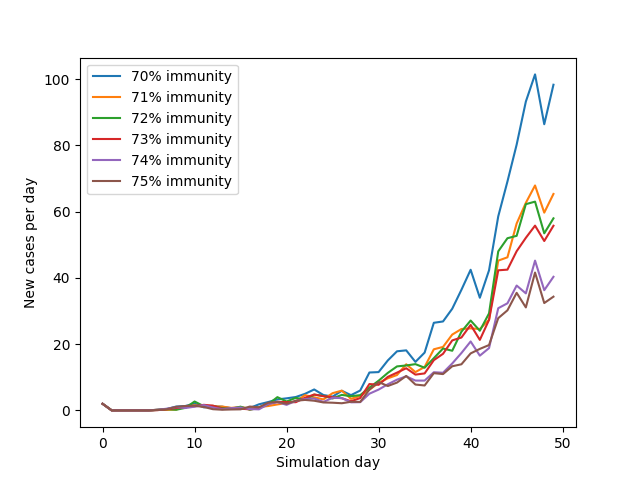
\includegraphics[width=\textwidth]{test_immunity_70-75.png}
	\caption{final estimate of outbreaks based on an average of 25 simulations}
\end{figure}
\newpage

\subsection{Estimating R\textsubscript{0}}
Here, we need to approximate the same graph but now he have to use an extra parameter, R\textsubscript{0}, the basic reproduction number of a disease, indicating how many people a single infected person will infect on average.
\\
\\
\noindent
We will use the same technique we used in the previous assignment, only this time, we need to repeat it for R0 = 12 .. 18.

\begin{table}
\begin{center}

	\begin{tabular}{c||c}
		R0 & estimated immunity rate \\ \hline
		12 & 65	\% \\
		13 & 68 \\
		14 & 69 \\
		15 & 70 \\
		16 & 73 \\
		17 & 74 \\
		18 & 76 \\
	\end{tabular}
	\caption{Estimated Immunity Rates based on 25 simulations}
	\end{center}

\end{table}

Generally speaking, the immunity rate is dependent of the parameter R0, which is to be expected. However, the parameter R0 doesn't seem to matter that much because the immunity rates are still pretty close to eachother.

\begin{figure}
	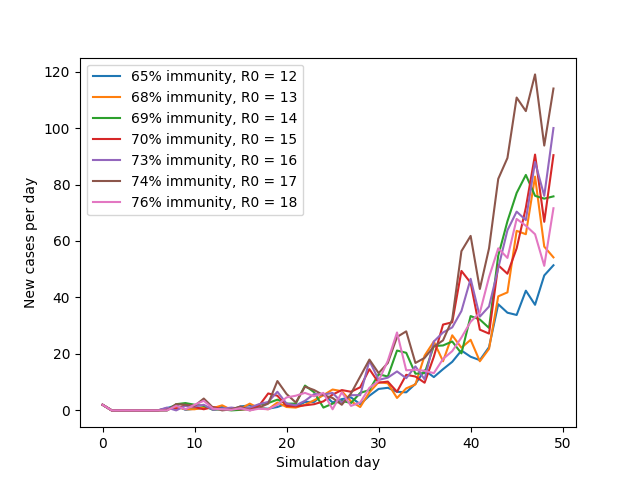
\includegraphics[width=\textwidth]{test_R0_final.png}
	\caption{25 simulations for found immunity values} 
\end{figure}

\newpage
\noindent
\section{Population generation}

\subsection{Investigating the influence of demography on epidemics}
We generate populations for two regions with different age distributions. We need to find which region is more likely to have an outbreak, region A, which has more younger people or region B, which has more elderly people. One might assume that the older region will have more chance because of the lower immunity the elderly might have.
\\
\\
\noindent
In case of population A there is around an 80\% chance for an outbreak to occur, in the simulations with population B there is 73\% chance for an outbreak. Population B is the older population in respect to population A, this means that an older population does not mean an increase in the likelihood of an outbreak, but a decrease. This could be explained by the fact that older people are commuting less.

\begin{figure}
	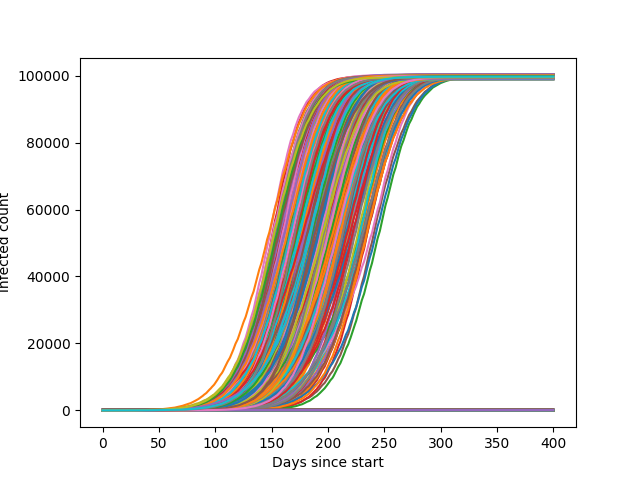
\includegraphics[width=\textwidth]{outbreaks_populationA.png}
	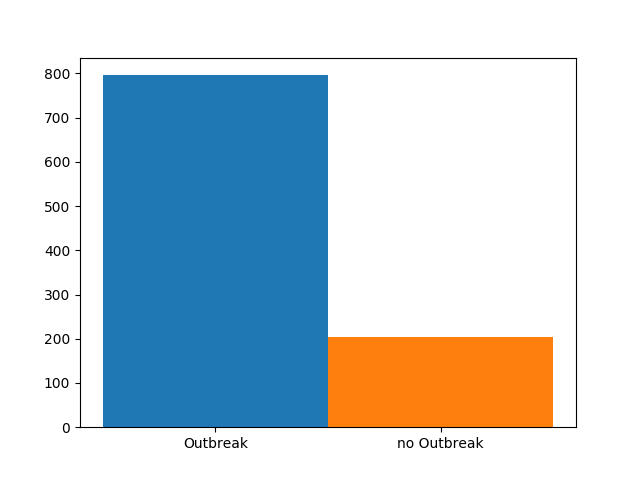
\includegraphics[width=\textwidth]{barchart_populationA.png}
	\caption{Results of 1000 simulations with population A}
\end{figure}
\begin{figure}
	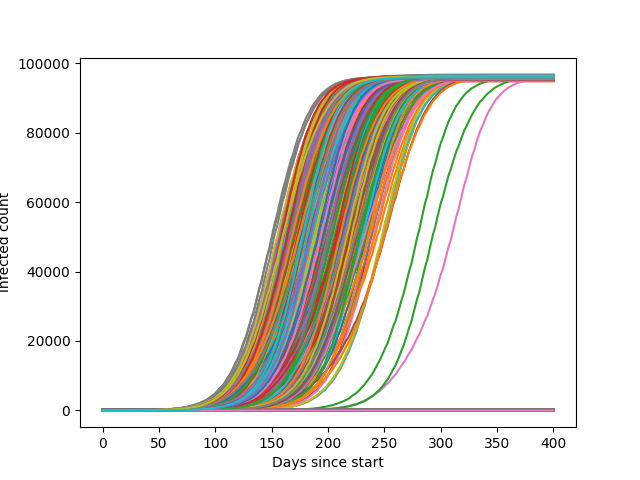
\includegraphics[width=\textwidth]{outbreaks_populationB.png}
	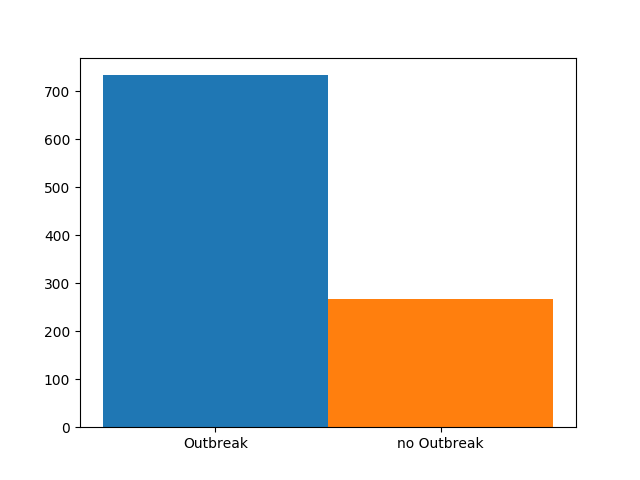
\includegraphics[width=\textwidth]{barchart_populationB.png}
	\caption{Results of 1000 simulations with population B}
\end{figure}
\newpage
\noindent
\subsection{Vaccinating on campus}
Vaccinations are often given at a young age. But not everyone gets vaccinated, there might be particular groups of people who are more susceptible. Here it is simulated what would happen if student were such a group. Their immunity will thus be lowered. To test if vaccinations during an outbreak aid in the surpression of it, two scenario's will be tested. One where the students aren't vaccinated and one where they are.\\
A total of 100 simulations have been run. 50 Without vaccinations and 50 with vaccinations given seven days after the first infected is introduced. A total of 1200 people will infected to start the outbreak. This is to make sure an outbreak will occur. The cumulative infected cases have been tracked from day to day and averaged over all simulations. The result is shown on fig \ref{vax_campus}. The results are averaged because there wasn't much deviation between the runs but a single run isn't a good representation.\\ \\
It is clear that even late vaccinations help in surpressing an outbreak. With only around 3500 students needing a vaccination in a studentbody of around 60000 and a total population of ten times that, the cost savinf is quite hight and the amount of infected is heavily reduced. \\
In conclusion, vaccinating students or people in general, who still need their vaccinations, is worth it during an outbreak.
 
\begin{figure}[h!]
	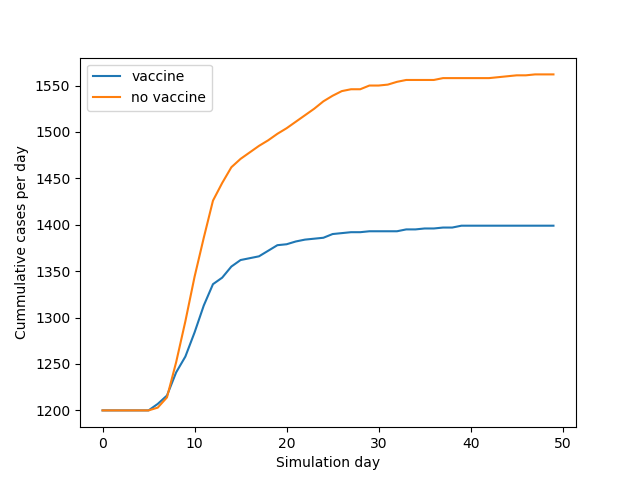
\includegraphics[width=\textwidth]{student_vaccinations.png}
	\caption{Above is a plot of average cumulative cases of 50 simulation each seen day by day. The student have a lowered immunity against the disease. During the blue scenario the students are vaccinated after seven days. They are not in the orange scenario.}
	\label{vax_campus}
\end{figure}
\newpage

\subsection{Is commuting to work important for disease spread?}
One could easily assume that working at a different location affects the rate at which a disease spreads, as it enhances it's reach. In a first simulation we generated simulations for 5 different commuting percentages. As you can clearly see, it does affect the rate at which the disease spreads, but it has no, or little, effect on whether the disease does or does not spread. In all cases, the entire population got the disease, be it that it took a few days longer to get to that point. Another thing we can remark is that the highest "peak" of newly diseased people is lower the lower the commuting factor gets. A possible cause of the lack of serious effect can come from the fact there are a lot of college commuters who will have the same effect as the workplace commuters. 

\begin{figure}
	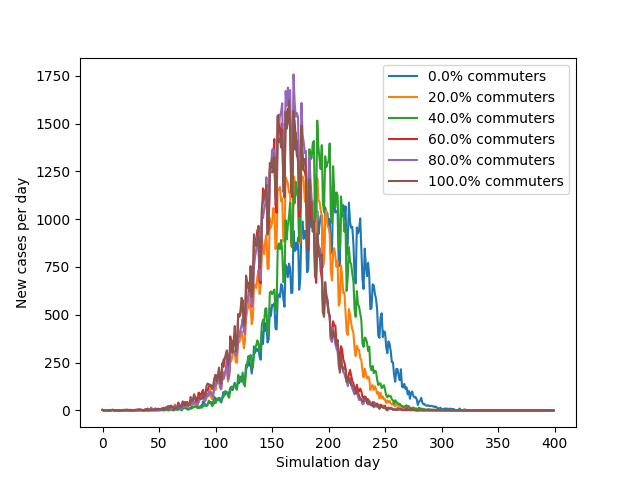
\includegraphics[width=\textwidth]{test_0-100.png}
	\caption{Results of 6 different percentages of commuters in a range from 0 to 100.}
\end{figure}
\newpage

If you watch the top of the graph, you can see that from a certain fraction and onwards, there is little to no difference in their behavior. To get a better view we graphed a closeup of percentages between 30 and 70. In the next graph you can see that the peeks are almost equally in height. You can even notice that some of the higher percentages have their peeks later then the ones with a lower percentage. 
\begin{figure}
	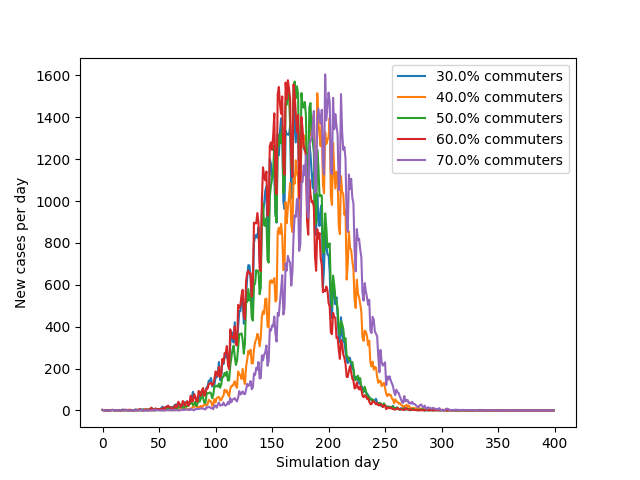
\includegraphics[width=\textwidth]{test_30-70.png}
	\caption{Results of 5 different percentages of commuters in a range from 30 to 70.}
\end{figure}
\\
Considering the recorded data we can see that solely changing the percentage of people who commute to work will not affect the spreading of disease in a significant manner. The disease will still spread all the same, but at a slower pace. 

\newpage
\section{Performance profiling of sequential code}
To study the performance of the code we will discuss a few parameters. We used the GPROF tool to profile the code. Based on these result we could see the influence of different parameters on the runtime.
\\
First we will choose a random number of days to run a simulation and look at the time needed to complete the algorithm. We considered in total 19 different amount of days in an interval of 10 to 2000 days. \\ 
\\
As could be expected, there is an increase in execution time when we take a larger amount of days. The number of days determines the number of loops in a simulation, hence this logically affects the needed time for a simulation by quite a big margin. This parameter will cause the largest change in perfomance in comparison with the other ones. Especially the sorting of the members en getting the total amount of infected people took up most of the computing time.

\begin{table}
\caption{Relation between the number of days and the runtime}
\begin{center}
	\begin{tabular}{ | c | c |}
	\hline
	Number of days & Time needed \\ \hline
	10 & 00:00:03:946:037 \\ \hline
	50 & 00:00:06:885:956 \\ \hline
	100 & 00:00:10:964:261 \\ \hline
	500 & 00:00:36:137:411 \\ \hline
	1000 & 00:01:07:248:430 \\ \hline
	2000 & 00:02:06:124:493 \\
	\hline	
	\end{tabular}
\end{center}
\end{table}

\noindent
Next, we vary the parameter of population size. From the following table it is clear that the larger the population the longer the simulation needs to finish. From the GPROF analysis we notice that the most work is done in getting the count of the infected and soritng the members. It can be said that the size of the population delivers the most influence on the total time. One can argue that the number of days had the most impact but it is not completely realistc to study outbreaks over a number of years what takes up the most computation time. A larger population is more common than a large number of days.
\\
In the previous part we considered the impact of the number of days. And as could be expected a large number of days combined with a large population will result in a large execution time.

\begin{table}
	\caption{Relation between population size and simulation runtime with 50 days}
\begin{center}
	\begin{tabular}{ | c | c |}
		\hline
		Population size & Time needed \\ \hline
		1000 & 00:00:00:429:476 \\ \hline
		50000 & 00:00:00:620:702 \\ \hline
		100000 & 00:00:00:954:298 \\ \hline
		500000 & 00:00:03:904:541 \\ \hline
		1000000 & 00:00:07:272:251 \\
		\hline	
	\end{tabular}
\end{center} 
\end{table}
\newpage
\noindent
When considering the time needed to generate a geo-based population and write it to a file without performing a simulation, the tendency of an increasing time with a larger population can be observed. The most computingpower went to writing the contact pools for the population.
\begin{table}
	\caption{Relation between population size and generating runtime with 50 days}
	\begin{center}
		\begin{tabular}{ | c | c |}
			\hline
			Population size & Time needed \\ \hline
			1000 & 00:00:00:262:863 \\ \hline
			10000 & 00:00:00:308:607 \\ \hline
			100000 & 00:00:00:336:115 \\ \hline
			500000 & 00:00:01:130:983 \\ \hline
			1000000 & 00:00:02:386:551 \\
			\hline
		\end{tabular}
	\end{center}
\end{table}

\noindent
When varying the immunity rate, there is no significant difference in runtime for different configurations. In order for this variable to have an influence on the final result, it is necessary to give other parameters different values.  As mentioned earlier, most of the time is used to sort and analyze the population, a factor like immunity rate has no effect on this process. In the table below you can see the runtimes for different immunity rates and a period of 50 days. When performing this ananlysis with a higher number of days of course this took some more time. But changing the immunity itself has no effect.

\begin{table}
	\caption{Relation between immunity rate and runtime for a 50 days}
\begin{center}
	\begin{tabular}{ | c | c |}
		\hline
		Immunity rate & Time needed \\ \hline
		0.2 & 00:00:04:869:367 \\ \hline
		0.4 & 00:00:04:873:811 \\ \hline
		0.6 & 00:00:04:966:409 \\ \hline
		0.8 & 00:00:05:035:361 \\ \hline
		0.99 & 00:00:04:921:399 \\
		\hline	
	\end{tabular}
\end{center}
\end{table}
 
\noindent
Seeding rate has a slight impact, but this impact is minimal. Seeding rate has no effect on the computation needed to sort and analyze the population, which is the major faction in a simulation. The following observations were made with a number of days equal to 50. A larger amount 
\begin{table}
\caption{Relation between the seeding rate and the runtime}
\begin{center}
	\begin{tabular}{ | c | c |}
		\hline
		Seeding rate & Time needed \\ \hline
		0.000001 & 00:00:06:210:017 \\ \hline
		0.00001 & 00:00:06:188:449 \\ \hline
		0.0001 & 00:00:06:294:636 \\ \hline
		0.001 & 00:00:06:659:908 \\ \hline
		0.01 & 00:00:07:437:776 \\ \hline
		0.1 & 00:00:07:406:320 \\
		\hline	
	\end{tabular}
\end{center} 
\end{table} 
\noindent

The contact log mode has a significant impact on the running time of a simulation. When the standard algorithm is used (all or susceptibles) it requires a lot more time to complete the simulation. It forms a large contrast with the running time needed when using the optimized algorithm with all the members of the contact pool sorted. By reducing the number of loops in the algorithms, the necessary time to complete the algorithm can be reduced along with it.
\begin{table}
	\caption{Relation between the contact log mode and time needed to perform a simulation with 50 days.}
\begin{center}
	\begin{tabular}{ | c | c |}
		\hline
		Contact log mode & Time needed \\ \hline
		All & 00:18:38:106:723 \\ \hline
		Susceptibles & 00:18:20:352:080 \\ \hline
		None & 00:00:06:620:969 \\ \hline
		Transmissions & 00:00:06:793:748 \\
		\hline	
	\end{tabular}
\end{center}
\end{table}

\subsection{Conclusion}
In general we can conclude that there are three parameters that have quite an impact on the running time of a simulation: the size of the population, the amount of days and the algorithm that was used to run the simulation. The larger the size and the number of days, the longer it takes to complete one simulation. Thus in combination with various combinations of the other parameters the runtime can differ a lot.

\end{document}
